\documentclass[12pt, letterpaper]{article}
\usepackage{graphicx} % images
\usepackage[a4paper, left=2cm, right=2cm, top=2.5cm, bottom=2.5cm]{geometry}
\usepackage{amssymb}
\usepackage{amsmath}
\usepackage{gensymb}

\title{Analysis H Notes}
\author{Hayden L}
\date{2024-2025}

\begin{document}

\maketitle
\pagebreak

\section{Introduction}
These are my notes for Gunn High School Analysis Honors Course.
\pagebreak

\section{Geometric Approach to Matrices (GAtM)}
\subsection{Groups}\
\textbf{Group}: a set of elements with a binary operation (two inputs, one output)
\begin{enumerate}
    \item \textbf{Identity}: there is an identity element \(I \in G\), \(X \cdot I = I \cdot X = X\)
    \item \textbf{Inverse}: each element \(X\) has an inverse \(X^{-1}\) such that \(X \cdot X^{-1} = X^{-1} \cdot X = X\)
    \item \textbf{Associativity}: \(X \cdot (Y \cdot Z) = (X \cdot Y) \cdot Z\)
    \item \textbf{Closure}: If \(X \in G\) and \(Y \in G\), then \(X \cdot Y \in G\)
\end{enumerate}
\textbf{Order}: the number of elements in a finite group
\begin{itemize}
    \item \textbf{Snap Group} \(S_n\) (\(n\)-post snap group) has an order of \(n!\)
    \item \textbf{Dihedral Group} \(D_n\) (rotation and reflections of a regular \(n\)-gon) has an order of \(2n\)
    \item \textbf{Cyclic Group} \(C_n\) (rotation of a regular \(n\)-gon) has a order of \(n\)
\end{itemize}
\textbf{Period} of an element \(X\): the least possible integer \(n\) such that \(X^n = I\)\\
\textbf{Isomorphic} (Isomorphism of a group): two groups with the same order, inverse, periods, and table\\
\textbf{Generators} of a set are elements that can express \underline{all elements of a group} (also known as the smallest generating set).\\
\textbf{Subgroups}: elements in a group that are closed among themselves..

\subsection{Infinities and Infinite Groups}
\textbf{Countable Infinity}: numbers that can be put in one-to-one correspondence with the set of natural numbers \(\mathbb{N}\)\\
\textbf{Uncountable Infinity}: numbers that cannot be put in one-to-one correspondence with the set of natural numbers \(\mathbb{N}\)\\
\textbf{Cardinality}\footnote{Cardinality refers to the number of elements in a set, while isomorphism refers to the structure. Groups that are isomorphic have the same cardinality, but not all groups with the same cardinality are isomorphic.}: Two infinite sets have the same cardinality if their elements can be put into a one-to-one correspondence with each other.

\centering{\textbf{Number Sets}}
\begin{table}[h]
    \centering
    \begin{tabular}{|c|c|c|}
        \hline
        \textbf{Type of Number}  & \textbf{Definitions} & \textbf{Examples}  \\ \hline
        Natural Numbers \(\mathbb{N}\) & all positive integers from 1 to infinity & 1,2,3,... \\ \hline
        Integers \(\mathbb{Z}\) & a whole number that can be positive, negative, or zero  & ...,-1,0,1,...   \\ \hline
        Rational Numbers \(\mathbb{Q}\) &  numbers that can be expressed as a fraction  & \(\frac{2}{3}, 0.5\)   \\ \hline
        Irrational Numbers \(\mathbb{I}\) & numbers that cannot be expressed as a fraction & \(\sqrt{2}, \pi\)   \\ \hline
        Real Numbers \(\mathbb{R}\)  & the union of both rational and irrational numbers  & N/A  \\ \hline
        Imaginary Numbers & a square root of a negative number  & \(i\)  \\ \hline
        Complex Numbers \(\mathbb{C}\)  & the union of both real and imaginary numbers  & \(1+i\)  \\ \hline
    \end{tabular}
    \caption{Types of Numbers}
    \label{Table 1}
\end{table}
\pagebreak
\raggedright
Since not all infinities are equally big, we can prove that infinite sets have the same cardinality by:
\begin{enumerate}
    \item making a one-to-one correspondence between the sets, or 
    \item if you can prove that \(|A| \geq |B|\) and \(|A| \leq |B|\), then \(|A|=|B|\).\footnote{This means if you find two injective functions, \(f: A\rightarrow B\) and \(g: B\rightarrow A\), then there exists a bijective function \(h: A\rightarrow B\), according to the Cantor-Schroeder-Bernstein Theorem. }
\end{enumerate}
Comparing the set of standards for numbers, we get \[|\mathbb{N}|=|\mathbb{Z}|=|\mathbb{Q}|<|\mathbb{R}|=|\mathbb{C}|\] For example, we can prove that \underline{Natural Numbers and Integers} have the same cardinality (\(|\mathbb{N}|=|\mathbb{Z}|\)) by creating a one-to-one correspondence \[\mathbb{N}\quad\mathbb{Z}\] \[1\Leftrightarrow0\] \[2\Leftrightarrow1\] \[3\Leftrightarrow-1\] \[4\Leftrightarrow2\] \[5\Leftrightarrow-2\] \[...\] thus showing that \(\mathbb{N}\) and \(\mathbb{Z}\) have the same cardinality.
\vspace{1em}\\

We can also find a one-to-one correspondence between \underline{natural numbers and rational numbers} greater than zero.\\
\begin{figure}[h]
    \centering
    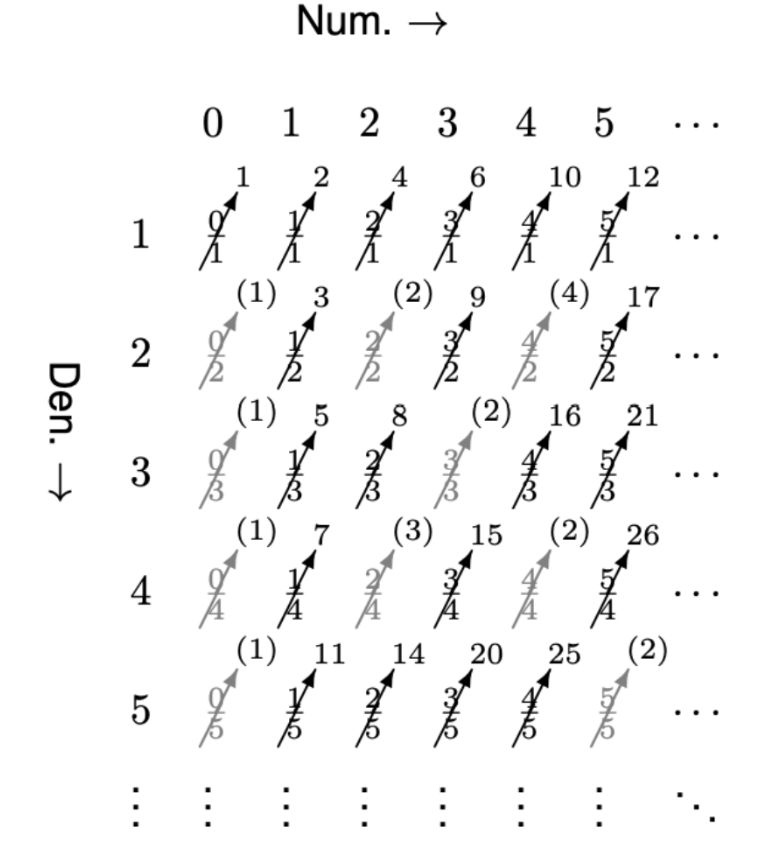
\includegraphics[width=0.45\textwidth]{images/naturalvsrational.png}\\
    \caption{Image 1: \( \mathbb{N} \) vs \( \mathbb{Q}_{\geq 0} \)}
    \label{fig: image1}
\end{figure}
\pagebreak

Now we can compare the infinite sets as listed on GAtM 5.9
\begin{table}[h]
    \centering
    \begin{tabular}{|c|l|c|l|}
        \hline
        & \textbf{Infinite Sets} & \textbf{Group?} & \textbf{Reason} \\ \hline
        a & natural numbers, addition & No & 0 not in group \\ \hline
        b & integers, addition & Yes & \\ \hline
        c & even integers, addition & Yes & \\ \hline
        d & odd integers, addition & No & odd + odd = even \\ \hline
        e & rational numbers, addition & Yes & \\ \hline
        f & real numbers, addition & Yes & \\ \hline
        g & complex numbers, addition & Yes & \\ \hline
        h & integers, multiplication & No & 0 has no identity \\ \hline
        i & integer powers of 2, multiplication & No & \\ \hline
        j & rational numbers, multiplication & No & 0 has no identity \\ \hline
        k & rational numbers excluding 0, multiplication & Yes & \\ \hline
        l & real numbers excluding 0, multiplication & Yes & \\ \hline
        m & complex numbers, multiplication & No & 0 has no identity \\ \hline
        n & rotation by a rational number of degrees & Yes & \\ \hline
        o & rotation by a rational number of radians & Yes & \\ \hline
        p & rotation by an integer number of radians & Yes & \\ \hline
    \end{tabular}
    \caption{Groups of Infinite Sets}
    \label{tab:groups_infinite_sets}
\end{table}\\
We can then see that groups b, c, i, and p are isomorphic to each other, groups e and o are isomorphic to each other, and groups f and g are isomorphic to each other.

\subsection{Geometry of Complex Numbers}
As a refresher of complex number terminology and notation:
\vspace{1em}\\

\textbf{Complex number in rectangular form}: \(z=a+bi\)\\
\textbf{Re(z)}: real part of \(z\), \(Re(z)=a\)\\
\textbf{Im(z)}: imaginary part of \(z\), \(Im(z)=b\)\\
\textbf{Arg(z)}: angle of \(z\) from the positive x-axis\\
\(|\)\textbf{z}\(|\): the length of \(z\), \(|z|=\sqrt{a^2+b^2}\)\\
\textbf{Conjugate of z}: \(\overline{z}=a-bi\)\\
\textbf{cis form}: \(z = |z| \, \text{cis} \, \theta \text{ or } z = r \, \text{cis} \, \theta, \text{where cis} \, \theta = \cos \theta + i \sin \theta\)
\vspace{1em}\\

Now, we can begin with De Moivre's Thereom, where \[(r \, \text{cis} \, \theta)^n = r^n \, \text{cis} \, (n\theta) \text{.}\] 
We can prove De Moivre's Theorem by showing \(r_1( \, \text{cos} \, A+i \, \text{sin} \, A)\cdot r_2( \, \text{cos} \, B+i \, \text{sin} \, B)\).\footnote{see slides}\footnote{Note that \(z\) and \(zi\) are always perpendicular.}
\vspace{1em}\\
\pagebreak

\textbf{\textit{n}-th roots of a complex number}: when finding the \(n\)-th roots of a complex number, you must make sure to find \underline{all} of the solutions. For instance, when finding \(\sqrt[n]{z}\), \[\sqrt[n]{z}\] \[=(r \, \text{cis} \, \theta)^{\frac{1}{n}}\] \[=r^{\frac{1}{n}} \, \text{cis} \, (\frac{\theta}{n}+\frac{2\pi k}{n})\] \[\text{for} \,k = 0,1,2,...,n-1\]
These \(n\) solutions are a result of the Fundamental Theorem of Algebra, which states that any polynomial of degree \(n\) has \(n\)-roots.

\subsection{Mapping the Plane with Matrices}
When mapping a matrices, consider a matrix representing a unit square \(M=
\begin{bmatrix}
0 & 1 & 1 & 0 \\
0 & 0 & 1 & 1
\end{bmatrix}\) and a transformation matrix. The following are a list of transformation matrices.\footnote{The identity, dilation, and some rotations and reflections have a corresponding complex number.} \vspace{1em}\\ 

\textbf{Identity}: \(
\begin{bmatrix} 
1 & 0 \\ 
0 & 1 
\end{bmatrix}\)\vspace{1em}\\

\textbf{Reflection over x-axis}: \(
\begin{bmatrix} 
1 & 0 \\ 
0 & -1 
\end{bmatrix}\)\vspace{1em}\\

\textbf{Reflection over y-axis}: \(
\begin{bmatrix} 
-1 & 0 \\ 
0 & 1 
\end{bmatrix}\)\vspace{1em}\\

\textbf{Reflection over line \textit{y=x}}: \(
\begin{bmatrix} 
0 & 1 \\ 
1 & 0 
\end{bmatrix}\)\vspace{1em}\\

\textbf{Rotation by \(\boldsymbol{\theta}\)}\footnote{Identical to multiplying by \(r \, \text{cis} \, \theta\).}: \(
\begin{bmatrix} 
\text{cos}\,\theta & -\text{sin}\,\theta \\ 
\text{sin}\,\theta & \text{cos}\,\theta 
\end{bmatrix}\)\vspace{1em}\\

\textbf{Stretch by \textit{k} in x-direction}: \(
\begin{bmatrix} 
k & 0 \\ 
0 & 1 
\end{bmatrix}\)\vspace{1em}\\

\textbf{Stretch by \textit{k} in y-direction}: \(
\begin{bmatrix} 
1 & 0 \\ 
0 & k 
\end{bmatrix}\)\vspace{1em}\\

\textbf{Shear\footnote{Shear is a type of linear transformation that distorts the shape of an object such that its points shift parallel to a given axis. Line that were originally parallel remain parallel and area remains the same, but angles between lines and lengths of line segments may change.} by \textit{k} in x-direction}: \(
\begin{bmatrix} 
1 & k \\ 
0 & 1 
\end{bmatrix}\)\vspace{1em}\\

\textbf{Shear by \textit{k} in y-direction}: \(
\begin{bmatrix} 
1 & k \\ 
0 & 1 
\end{bmatrix}\)\vspace{1em}\\

\textbf{Dilation with factor \textit{k}}: \(
\begin{bmatrix} 
k & 0 \\ 
0 & k 
\end{bmatrix}\)\vspace{1em}\\

\textbf{Translation by \(\boldsymbol{<\alpha,\beta>}\)}: \(
\begin{bmatrix} 
1 & 0 & \alpha \\ 
0 & 1 & \beta \\
0 & 0 & 1
\end{bmatrix}
\begin{bmatrix} 
x \\ 
y \\
1
\end{bmatrix}=
\begin{bmatrix}
x+\alpha \\
y+\beta \\
1
\end{bmatrix}\) \vspace{1em}\\

\textbf{Composite of two or more transformations}: When doing two or more transformations, the matrix written first is done second. Consider a rotation by \(90\degree\) and a reflection over the \(y\)-axis. If we were to do the reflection followed by the rotation, we would notate it \[R_{90\degree} \, r_y\text{,}\] while if we were to the rotation first, we would notate it \[r_y \, R_{90\degree}\text{.}\] The former order of transformations is identical to a reflection over the line \(y=-x\), where the latter is identical to a reflection over the line \(y=x\). You can also do a transformation with matrix \(\begin{bmatrix} 
a & b \\
c & d
\end{bmatrix}\) and translation by vector \(<\alpha,\beta>\) by using 3D matrices. Consider doing the transformation first to get \(\begin{bmatrix} 
1 & 0 & \alpha \\ 
0 & 1 & \beta \\
0 & 0 & 1
\end{bmatrix}
\begin{bmatrix} 
a & b & 0 \\ 
c & d & 0 \\
0 & 0 & 1
\end{bmatrix}
=
\begin{bmatrix} 
a & b & \alpha \\ 
c & d & \beta \\
0 & 0 & 1
\end{bmatrix}\).
\vspace{1em}\\

\textbf{Mapping points onto a line}: given a line \(ax+by=0\), we can use a matrix: \(
\begin{bmatrix} 
b & b \\ 
-a & -a 
\end{bmatrix}\) to map the points onto the line. To map the points onto a line \(y=\frac{a}{b}x+c\), we can use a 3D matrix.
\vspace{1em}\\

\textbf{Reflection over the line \(\boldsymbol{\theta=n\degree}\)} (i.e. line with equation \(y=x\,\text{tan}\,\theta)\): \(
\begin{bmatrix} 
\text{cos}2\theta & \text{sin}2\theta \\ 
\text{sin}2\theta & -\text{cos}2\theta 
\end{bmatrix}\).
\vspace{1em}\\
This can be derived from the fact that a composite of two reflections is a rotation, noting that the angle of the rotation is double the angle between the lines of reflection: \[r_{xtan\theta}\cdot r_x=R_{2\theta}\] \[r_{xtan\theta}\cdot r_x\cdot r_x^{-1}=R_{2\theta}\cdot r_x^{-1}\] \[r_{xtan\theta}=R_{2\theta}\cdot r_x^{-1}\] \[r_{xtan\theta}=R_{2\theta}\cdot r_x\]

\end{document}
